\documentclass[10pt, a4paper]{article}
\usepackage[utf8]{inputenc}
\usepackage{listings}
\usepackage{hyperref}

\usepackage{fancyhdr}
\pagestyle{fancy}
\lhead{PERALE Thomas et RUSU George}
\rhead{INFO-F-203}

\usepackage{graphicx}
\usepackage{tikz}
\usepackage{color} or \usepackage{xcolor}

\lstset{ %
backgroundcolor=\color{white},   % choose the background color; you must add \usepackage{color} or \usepackage{xcolor}
basicstyle=\footnotesize,        % the size of the fonts that are used for the code
breakatwhitespace=false,         % sets if automatic breaks should only happen at whitespace
breaklines=true,                 % sets automatic line breaking
captionpos=b,                    % sets the caption-position to bottom
commentstyle=\color{mygreen},    % comment style
deletekeywords={\ldots},            % if you want to delete keywords from the given language
escapeinside={\%*}{*)},          % if you want to add LaTeX within your code
extendedchars=true,              % lets you use non-ASCII characters; for 8-bits encodings only, does not work with UTF-8
frame=single,                      % adds a frame around the code
keepspaces=true,                 % keeps spaces in text, useful for keeping indentation of code (possibly needs columns=flexible)
keywordstyle=\color{blue},       % keyword style
language=Octave,                 % the language of the code
otherkeywords={*,\ldots},           % if you want to add more keywords to the set
numbers=left,                    % where to put the line-numbers; possible values are (none, left, right)
numbersep=5pt,                   % how far the line-numbers are from the code
numberstyle=\tiny\color{mygray}, % the style that is used for the line-numbers
rulecolor=\color{black},         % if not set, the frame-color may be changed on line-breaks within not-black text (e.g.  comments (green here))
showspaces=false,                % show spaces everywhere adding particular underscores; it overrides 'showstringspaces'
showstringspaces=false,          % underline spaces within strings only
showtabs=false,                  % show tabs within strings adding particular underscores
stepnumber=2,                    % the step between two line-numbers.  If it's 1, each line will be numbered
stringstyle=\color{mymauve}, % string literal style
tabsize=2, % sets default tabsize to 2 spaces
title=\lst
}

\begin{document}
\section{Description du problème}
    Dans un parking similaire à un est tableau de plusieurs cases,
    où chaques cases peut contenir soit une voiture qui peut avancer
    ou reculer selon son orientation (\emph{verticale} ou \emph{horizontale})
    soit un espace vide, déterminer pour une des voitures de ce parking
    (la voiture \emph{goal}) comment atteindre la sortie de ce parking en
    faisant bouger les voitures le moins possible.

\section{Cas de base.}
    Est fourni comme input pour le problême un fichier: \newline
    \lstinputlisting{../test/test1.txt}
    Il nous donne des informations sur:
    \begin{itemize}
        \item La taille du parking.
        \item La position de la sortie.
        \item L'emplacement des voitures dans ce parking.
    \end{itemize}
    Qui vont être parsé pour pouvoir créer un parking de base, qui est notre
    cas de base à partir duquel il va falloir trouver le plus court
    chemin.\newline
    Conformément à l'énoncé quelques l'algorithme ne va gèrer que les cas où:
    \begin{itemize}
        \item Le fichier d'input est correctement écrit (pas d'erreur dans
            celui-ci), à la même manière que dans l'exemple.
        \item La voiture goal se déplace horizontalement (la sortie est sur la
            droite ou la gauche).
        \item Il n'y a pas de voiture de taille 1 (car impossible de savoir si
            elle se déplace horizontalement ou verticalement).
        \item Pas de parking de taille 0 (car pas possible d'y mettre une
            voiture goal)
    \end{itemize}

\section{Description de la résolution du problême.}
    Le problême va se faire en plusieurs étapes:
    \begin{enumerate}
        \item Générer tout les configurations\footnote{Une configuration de
            parking est un parking avec les voitures à une certaine place.
            Quand on dit toutes les configurations possible on entend
            qu'à chaque fois qu'une voiture va bouger dans le parking on a une
            configuration différente.} de parking possible.
        \item Lors de cette génération, créer un graphe dans lequel chaques
            configurations nouvellement crée est lier à la configuration
            d'où elle vient.
        \item Une fois ces configurations générées, appliquer un algorithme de
            recherche du plus court chemin sur le graphe des configurations.
    \end{enumerate}

    Exemple\footnote{Les exemples sont créés à partir de
    http://analogbit.com/software/puzzletools/ .} de graphe associer aux
    configurations lors d'une génération non exhaustive (on abouti à deux
    situation gagnant2).\newline

    % 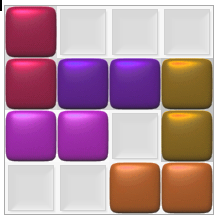
\includegraphics[scale=0.2]{gen0.png} \newline
    % \newpage
    \begin{tikzpicture}
        [scale=.8,auto=left,every node/.style={circle,fill=blue!20}]
        \node (n0) at (1, 10) {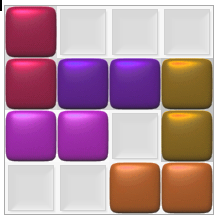
\includegraphics[scale=0.15]{gen0.png}};
        \node (n1) at (4, 10) {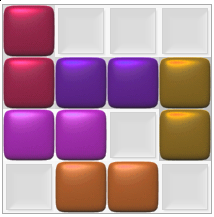
\includegraphics[scale=0.15]{gen1.png}};
        \node (n2) at (7, 10) {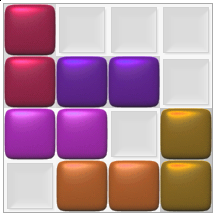
\includegraphics[scale=0.15]{gen2.png}};
        \node (n3) at (10, 10) {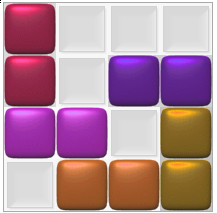
\includegraphics[scale=0.15]{gen3.png}};
        % Premier win

        %Autre situation à partir de n0
        \node (n4) at (1, 7) {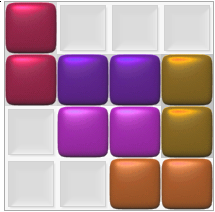
\includegraphics[scale=0.13]{gen4.png}};
        \node (n5) at (2, 5) {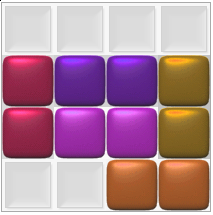
\includegraphics[scale=0.13]{gen5.png}};
        \node (n6) at (4, 4) {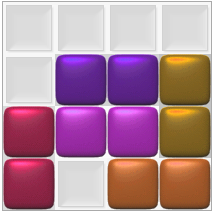
\includegraphics[scale=0.13]{gen6.png}};
        \node (n7) at (7, 4) {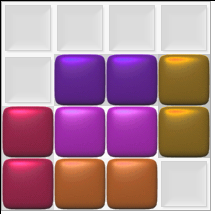
\includegraphics[scale=0.13]{gen7.png}};
        \node (n8) at (10, 4) {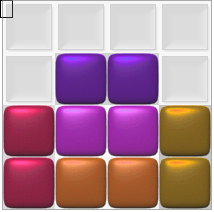
\includegraphics[scale=0.13]{gen8.png}};
        \node (n9) at (13, 4) {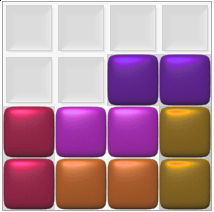
\includegraphics[scale=0.13]{gen9.png}};

        \node (n10) at (13, 4) {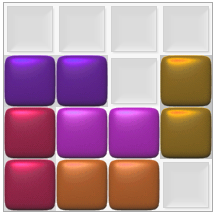
\includegraphics[scale=0.13]{gen10.png}};

        \foreach \from/\to in {n0/n1, n1/n2, n2/n3, n0/n4, n4/n5, n5/n6, n6/n7,
        n7/n8, n8/n9}
        \draw (\from) -- (\to);
    \end{tikzpicture}

\subsection{Génération des configurations.}
    Pour générer l'ensemble des solutions un algorithme de backtracking est
    utilisé, il fait avancer/reculer un maximum chaques voitures dans chaques
    configuration que cela va engendrer.
\subsection{Recherche du plus court chemin.}
    Pour trouver le plus court chemin parmis ceux générés. L'algorithme le plus
    évident pour effectuer un tel travail est l'algorithme de Dijkstra.
    Or ici nous avons un cas spécial de
    l'algorithme de Dijkstra car la distance entre chaques noeuds est de 1, là
    où l'algorithme de Dijkstra fait une recherche dans un graph où
    la distance entre deux noeuds est à chaques fois différente.
    Ainsi la \emph{min-priority queue} n'est pas nécessaire, une simple
    \emph{queue} peut être utilisé.
    L'algorithme ressemble donc à un parcour en largeur (\emph{breadth-first})
    qui s'arrête au premier parking \emph{gagnant} rencontré. \newline

    Exemple en mettant en évidence les profondeurs du parcour: \newline
    \begin{tikzpicture}
        [scale=.8,auto=left,every node/.style={circle,fill=blue!20}]
        \node (n0) at (1, 10) {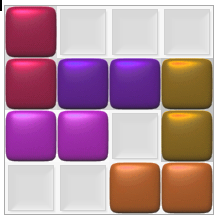
\includegraphics[scale=0.15]{gen0.png}};
        \node (n1) at (4, 10) {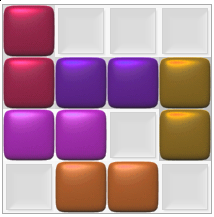
\includegraphics[scale=0.15]{gen1.png}};
        \node (n2) at (7, 10) {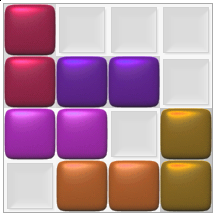
\includegraphics[scale=0.15]{gen2.png}};
        \node[color=green] (n3) at (10, 10) {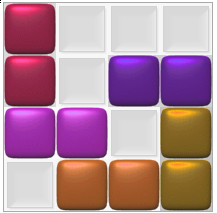
\includegraphics[scale=0.15]{gen3.png}};
        % Premier win

        %Autre situation à partir de n0
        \node (n4) at (1, 7) {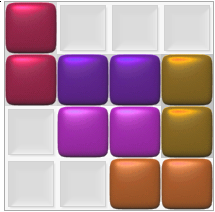
\includegraphics[scale=0.13]{gen4.png}};
        \node (n5) at (2, 5) {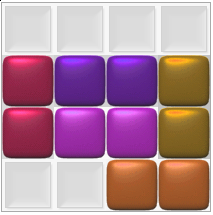
\includegraphics[scale=0.13]{gen5.png}};
        \node (n6) at (4, 4) {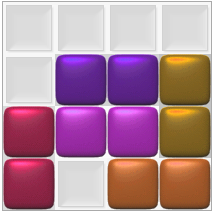
\includegraphics[scale=0.13]{gen6.png}};
        \node (n7) at (7, 4) {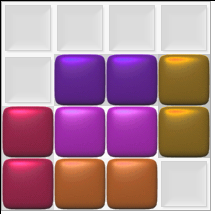
\includegraphics[scale=0.13]{gen7.png}};
        \node (n8) at (10, 4) {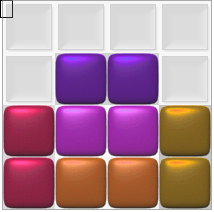
\includegraphics[scale=0.13]{gen8.png}};
        \node (n9) at (13, 4) {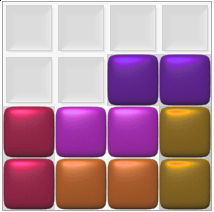
\includegraphics[scale=0.13]{gen9.png}};

        \node (n10) at (13, 4) {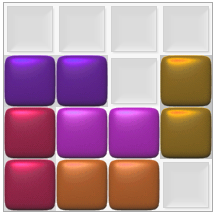
\includegraphics[scale=0.13]{gen10.png}};

        \foreach \from/\to in {n0/n1, n1/n2, n2/n3, n0/n4, n4/n5, n5/n6, n6/n7,
        n7/n8, n8/n9}
        \draw (\from) -- (\to);
        \draw[color=red]  (1, 8) to[out=10,in=-90] (3, 10);
        \draw[color=red]  (1, 6) to[out=0,in=-85] (5, 10);
        \draw[color=red]  (3, 5) to[out=90,in=-85] (8, 10);
        \draw[color=red] (6, 4) to[out=90,in=-85] (11, 10);
    \end{tikzpicture}



\section{Optimisation}
\begin{thebibliography}
\bibitem{Rush Hour and Dijkstra's algorithm}
    Mark Stamp, Brad Engel McIntosh Ewekk, Victor Morrow,
    \emph{Rush Hour and Dijkstra's algorithm}
    http://www.cs.sjsu.edu/~stamp/cv/papers/rh.pdf

\end{thebibliography}

\end{document}
